\subsubsection{FC Portugal} \label{fc_portugal}

Portugalský tím FC Portugal\cite{fc_portugal}.
Navrhli metódu pre kopanie do viacerých smerov. Je zložený z troch častí. 

Prvou je vytvorenie dráhy, akou musí smerovať noha robota, aby sa lopta dostala do želaného smeru. Na vytvorenie krivky pohybu nohy použili Bezierovu rovnicu tretieho stupňa. 

Druhou časťou je modul pre inverznú kinematiku, ktorý na základe predtým vypočítanej krivky vypočíta natočenie kĺbov pre vykonanie kopu. 

Posledná časť je stabilizačný modul, ktorý sa snaží dosiahnuť to, aby sa ťažisko robota nachádzalo v ploche druhej podpornej nohy. Do fázy stabilizovania vstupujú aj horné končatiny, ktoré sa upažia alebo predpažia. V extrémnom prípade, ak nestačí pohybovanie rukou, upravuje sa pozícia bokov, členkov a robot sa predkláňa na vyrovnanie stability. Avšak kop nie je dostatočne stabilný. Neriešili parametrizovanie vzdialenosti pri kope.
%Vo výsledkoch boli úspešní pri vypočítavaní krivky (jednoduchý matematický výpočet). Taktiež výsledky dosiahli, že robot kopol loptu do požadovaného smeru. Očakávania nenaplnili pri dosahovaní stability kopu. Neriešili parametrizovanie vzdialenosti.

\begin{figure}[H]
	\center
	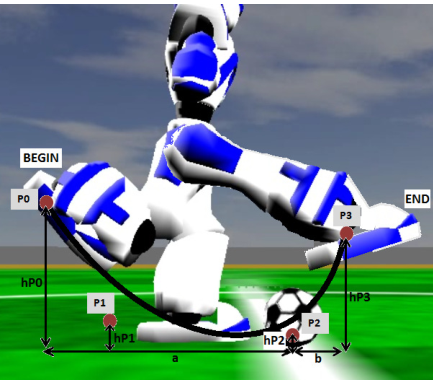
\includegraphics[scale=1]{./data/kick_arch_fc_portugal}
	\caption{Schéma kopu tímu FC Portugal \cite{fc_portugal}}
	\label{pic_kick_arch_fc_portugal}
\end{figure}


\begin{algorithm}
	\caption{Implementácia všesmerového kopu FC Portugal}\label{} 
	\begin{algorithmic}
		\STATE \texttt{foot = chooseFoot()}
		\STATE \texttt{P0, P1, P2, P3 = computeBezierParamters(ball, target, a, b)}
		\FOR {\texttt{i := 1} \TO \texttt{nTrajPoints}}
			\STATE \texttt{trajPoint = computeCurvePoint(P0, P1, P2, P3, nTrajPoints)}
			\STATE \texttt{H = determineRotTransMatrix(trajPoint)}
			\STATE \texttt{joints = computeInverseKinematics(H, foot)}
			\STATE \texttt{joints = computeStability(joints)}
			\STATE \texttt{slots = addSlot(joints, duration)}
		\ENDFOR
		\STATE \texttt{performMovement(slots)}
	\end{algorithmic}
\end{algorithm}

Pohyb začína výberom nohy, ktorou sa bude kopať. Pre výber nohy sa berie do úvahy vzdialenosť od lopty. Pokračuje sa určením parametrov pre Bezierovu krivku, ktorá bude vyjadrovať dráhu pre nohu. Kde vstupné hodnoty do kubickej rovnice Bezierovej krivky pre 4 kontrolné body (\ref{eq_bezier}) vyjadruje obrázok \ref{pic_kick_arch_fc_portugal_params}, kde $t \in [0,1]$.
\begin{equation}\label{eq_bezier}
	b(t) = \sum_{i = 0}^{3}
	{
		{3 \choose i} t^i {(1 - t)}^{3 - i} P_i
	}
\end{equation}

\begin{figure}[H]
	\center
	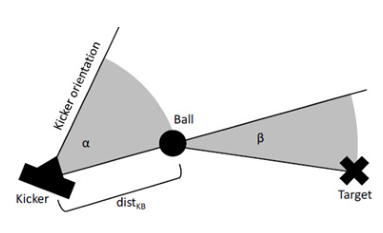
\includegraphics[scale=1]{./data/kick_arch_fc_portugal_params}
	\caption{Parametre potrebné pre výpočet kontrolných bodov krivky všesmerového kopu \cite{fc_portugal}}
	\label{pic_kick_arch_fc_portugal_params}
\end{figure}

Medzi vstupné parametre patrí pozícia lopty a cieľa a tiež uhol medzi vektorom vyjadrujúcim smer natočenia hráča a vektorom spájajúcim pozíciu hráča a pozíciu lopty a nakoniec uhol medzi vektorom hráčovej nohy a lopty a vektorom od lopty k cieľu. Krivka je potom rozdelená na $n$ bodov. Pre každý z nich:

\begin{itemize}
 \item vypočíta pozícia v priestore
 \item určí sa homogénna matica, ktorá obsahuje natočenia a pozíciu nohy vzhľadom na panvu
 \item vypočítajú sa natočenia pre kĺby pomocou inverznej kinematiky
 \item upravia sa hodnoty kĺbov kvôli stabilizovaniu robota
\end{itemize}
Každý takýto výpočet zodpovedá jednej fáze pohybu. Nakoniec sa vykoná pohyb zo všetkých vypočítaných fáz.